%%%%%%%%%%%%%%%%%%%%%%%%%%%%%%%%%%%%%%%%%%%%%%%%%%%%%%%%%%%%%%%%%%%%%%%%%%
\begin{table*}[tbp!]
%\vspace{-1mm}
\centering
{\small 
\begin{tabular}{|l|r|r|r|r|l|} \hline
Dataset & \# Features & \# Data & \# Features/\# Data & \% True Labels & Feature Type\\ \hline \hline 
Breast Cancer(BC)	& 9	& 699	& 0.013	& 34 \%	& All Numeric\\ \hline
Diabetes(D)        & 8	& 768	& 0.010	& 35 \%	& All Numeric\\ \hline
Heart Statlog(HS)	& 13	& 270	& 0.048	& 44 \%	& All Numeric\\ \hline
Spect(S)	        & 22	& 80	& 0.275 & 33 \%	& Categorical\\ \hline
Vote(V)	        & 16	& 435	& 0.037	& 39 \%	& Categorical\\ \hline
Newsgroup(NG)	& 500	& 1963	& 0.255	& 49 \%	& All Binary\\ \hline
Horse Colic(HC)	& 22	& 368	& 0.060	& 37 \%	& Categorical (16) and numeric (6)\\ \hline
Credit-American(CR)	& 15	& 690	& 0.022	& 44 \%	& Categorical(9) and numeric (6)\\ \hline
Credit-German(GC)	& 20	& 1000	& 0.020 & 30 \%	& Categorical (13) and Numeric (7)\\ \hline
Hepatitis(H)	& 19	& 155	& 0.123	& 21 \%	& Categorical (13) and Numeric (6)\\ \hline
Ionosphere(I)	& 34	& 351	& 0.097	& 36 \%	& All Numeric\\ \hline
%KR-vs-KP	& 36	& 3196	& 0.011	& 48 \%	& All Categorical\\ \hline
%Labor	        & 16	& 57	& 0.281	& 35 \%	& Categorical (8) and Numeric (8)\\ \hline
%Mushroom	& 22	& 8124	& 0.003	& 48 \%	& All Categorical\\ \hline
%Sick	        & 29	& 3772	& 0.008	&  6 \%	& Categorical (23) and Numeric (6)\\ \hline
%Sonar	        & 60	& 208	& 0.288 & 47 \%	& All Numeric\\ \hline
\end{tabular}}
\vspace{-1mm}
\caption{\footnotesize Descriptive statistics of the various datasets evaluated in this work.}
\label{table:stats}
\vspace{-4mm}
\end{table*}
%%%%%%%%%%%%%%%%%%%%%%%%%%%%%%%%%%%%%%%%%%%%%%%%%%%%%%%%%%%%%%%%%%%%%%%%%%

%%%%%%%%%%%%%%%%%%%%%%%%%%%%%%%%%%%%%%%%%%%%%%%%%%%%%%%%%%%%%%%%%%%%%%%%%%
\begin{figure*}[tbp!]
\includegraphics[width=0.85\textwidth]{./figures/dataset_perf/Accuracy.pdf}\\
\includegraphics[width=0.85\textwidth]{./figures/dataset_perf/Recall.pdf}
\includegraphics[width=0.10\textwidth]{./figures/dataset_perf/legend.PNG}
\vspace{-2mm}
\caption{\footnotesize Performance of various feature selection algorithms per dataset, averaged across classifier type and each stage of feature selection.  Overall the newly proposed CVL method performs well on Recall on most datasets, while the Recall performance of other feature selection algorithms vary; interestingly the best performance is achieved for datasets a high ratio of features to data indicating that the strong conjunctive voting scheme of CVL may help reduce noise in feature selection for these datasets. }
\label{fig:perf_vs_dataset}
\vspace{-4mm}
\end{figure*}
%%%%%%%%%%%%%%%%%%%%%%%%%%%%%%%%%%%%%%%%%%%%%%%%%%%%%%%%%%%%%%%%%%%%%%%%%%

%%%%%%%%%%%%%%%%%%%%%%%%%%%%%%%%%%%%%%%%%%%%%%%%%%%%%%%%%%%%%%%%%%%%%%%%%%
\begin{figure*}[tbp!]
\centering
\includegraphics[width=0.42\textwidth]{./figures/class_perf/Accuracy.pdf}
\includegraphics[width=0.42\textwidth]{./figures/class_perf/Recall.pdf}
\includegraphics[width=0.15\textwidth]{./figures/class_perf/legend.PNG}
\vspace{-6mm}
\caption{\footnotesize Performance of various feature selection algorithms per classifier, averaged across dataset and each stage of feature selection.  DVE, DVL, CVE, and CVL align with the independence assumptions of Naive Bayes and the maximum (conditional) likelihood framework of Naive Bayes and Logistic Regression, which may explain the better excellent performance of these algorithms with these classifiers.}
\label{fig:perf_vs_classifier}
\end{figure*}
%\vspace{-6mm}
%%%%%%%%%%%%%%%%%%%%%%%%%%%%%%%%%%%%%%%%%%%%%%%%%%%%%%%%%%%%%%%%%%%%%%%%%%

%%%%%%%%%%%%%%%%%%%%%%%%%%%%%%%%%%%%%%%%%%%%%%%%%%%%%%%%%%%%%%%%%%%%%%%%%%
\begin{figure*}[tbp!]
\centering
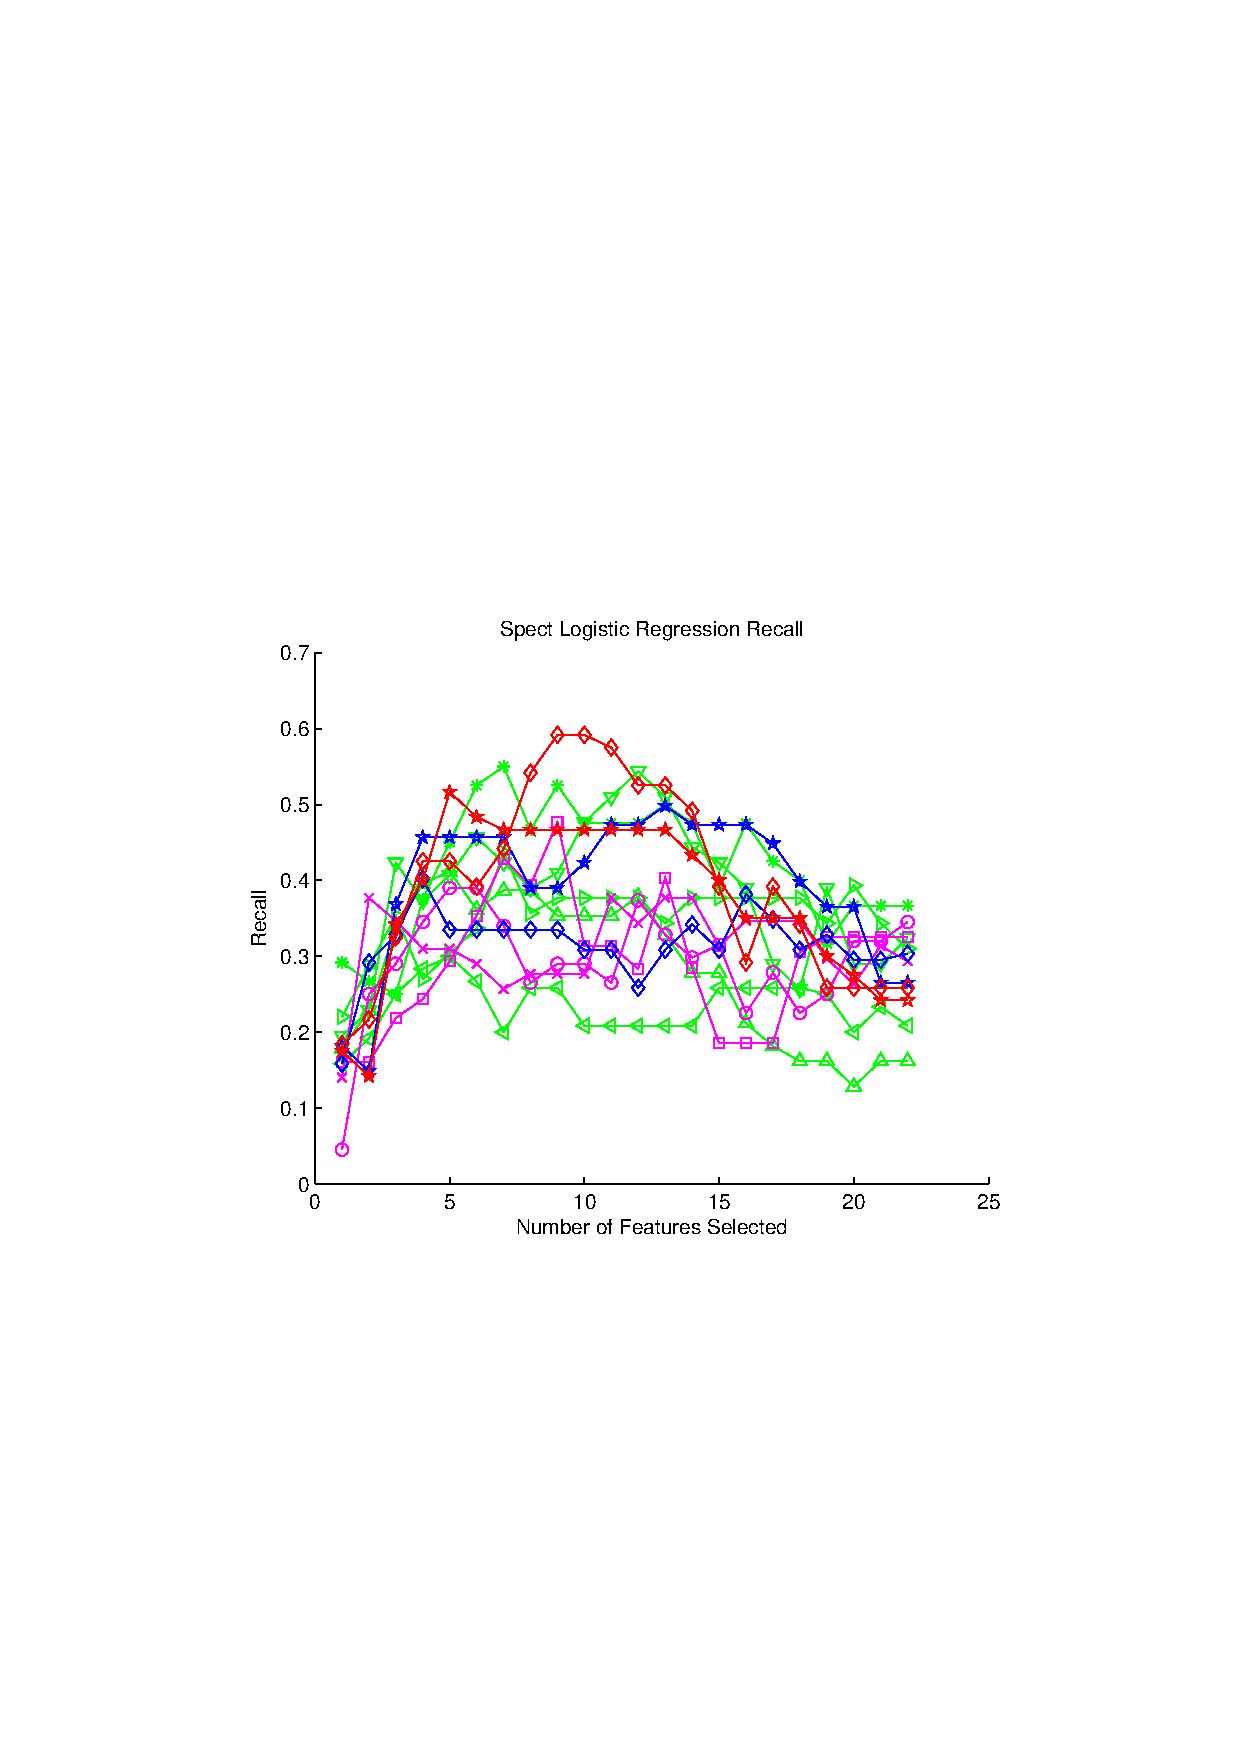
\includegraphics[width=0.375\textwidth]{./figures/linegraphs/SpectLogisticRegressionRecall.pdf}
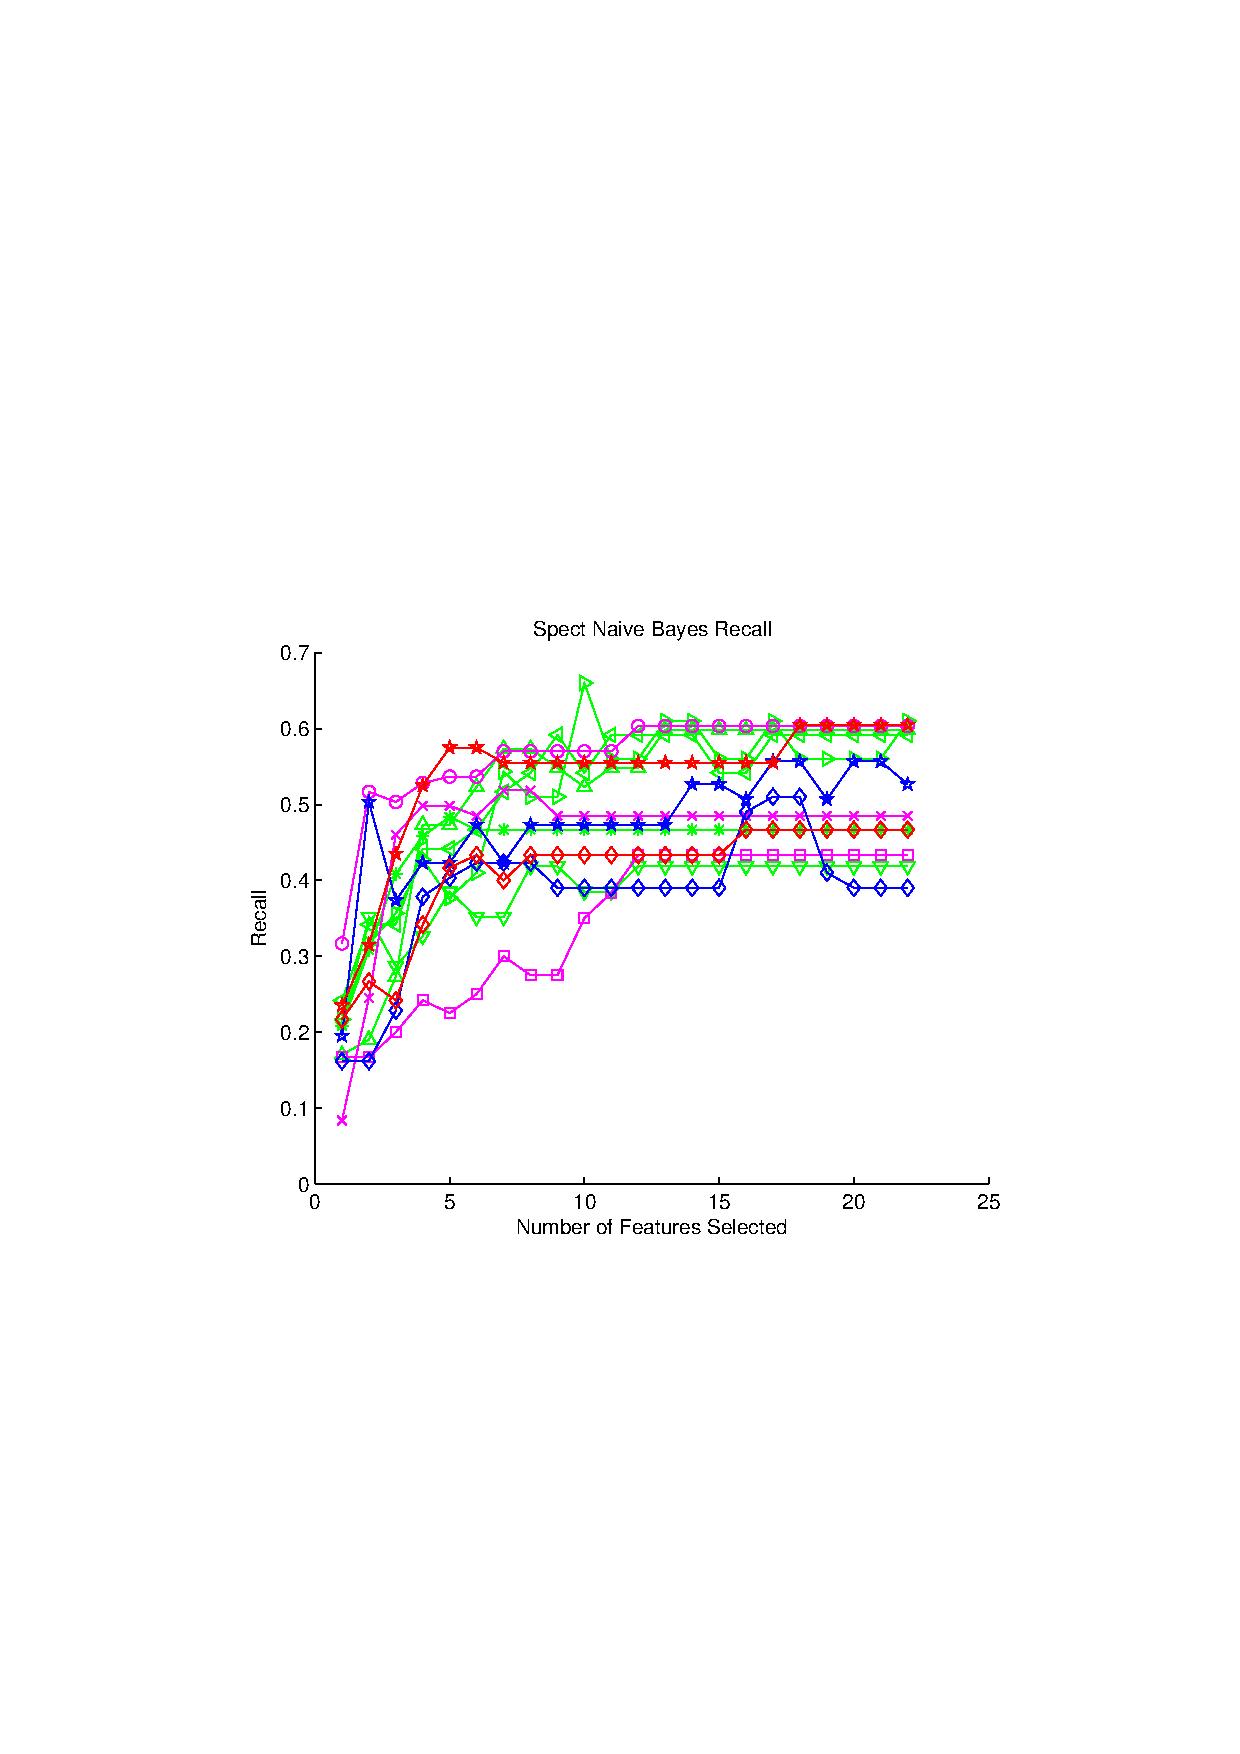
\includegraphics[width=0.375\textwidth]{./figures/linegraphs/SpectNaiveBayesRecall.pdf}\\
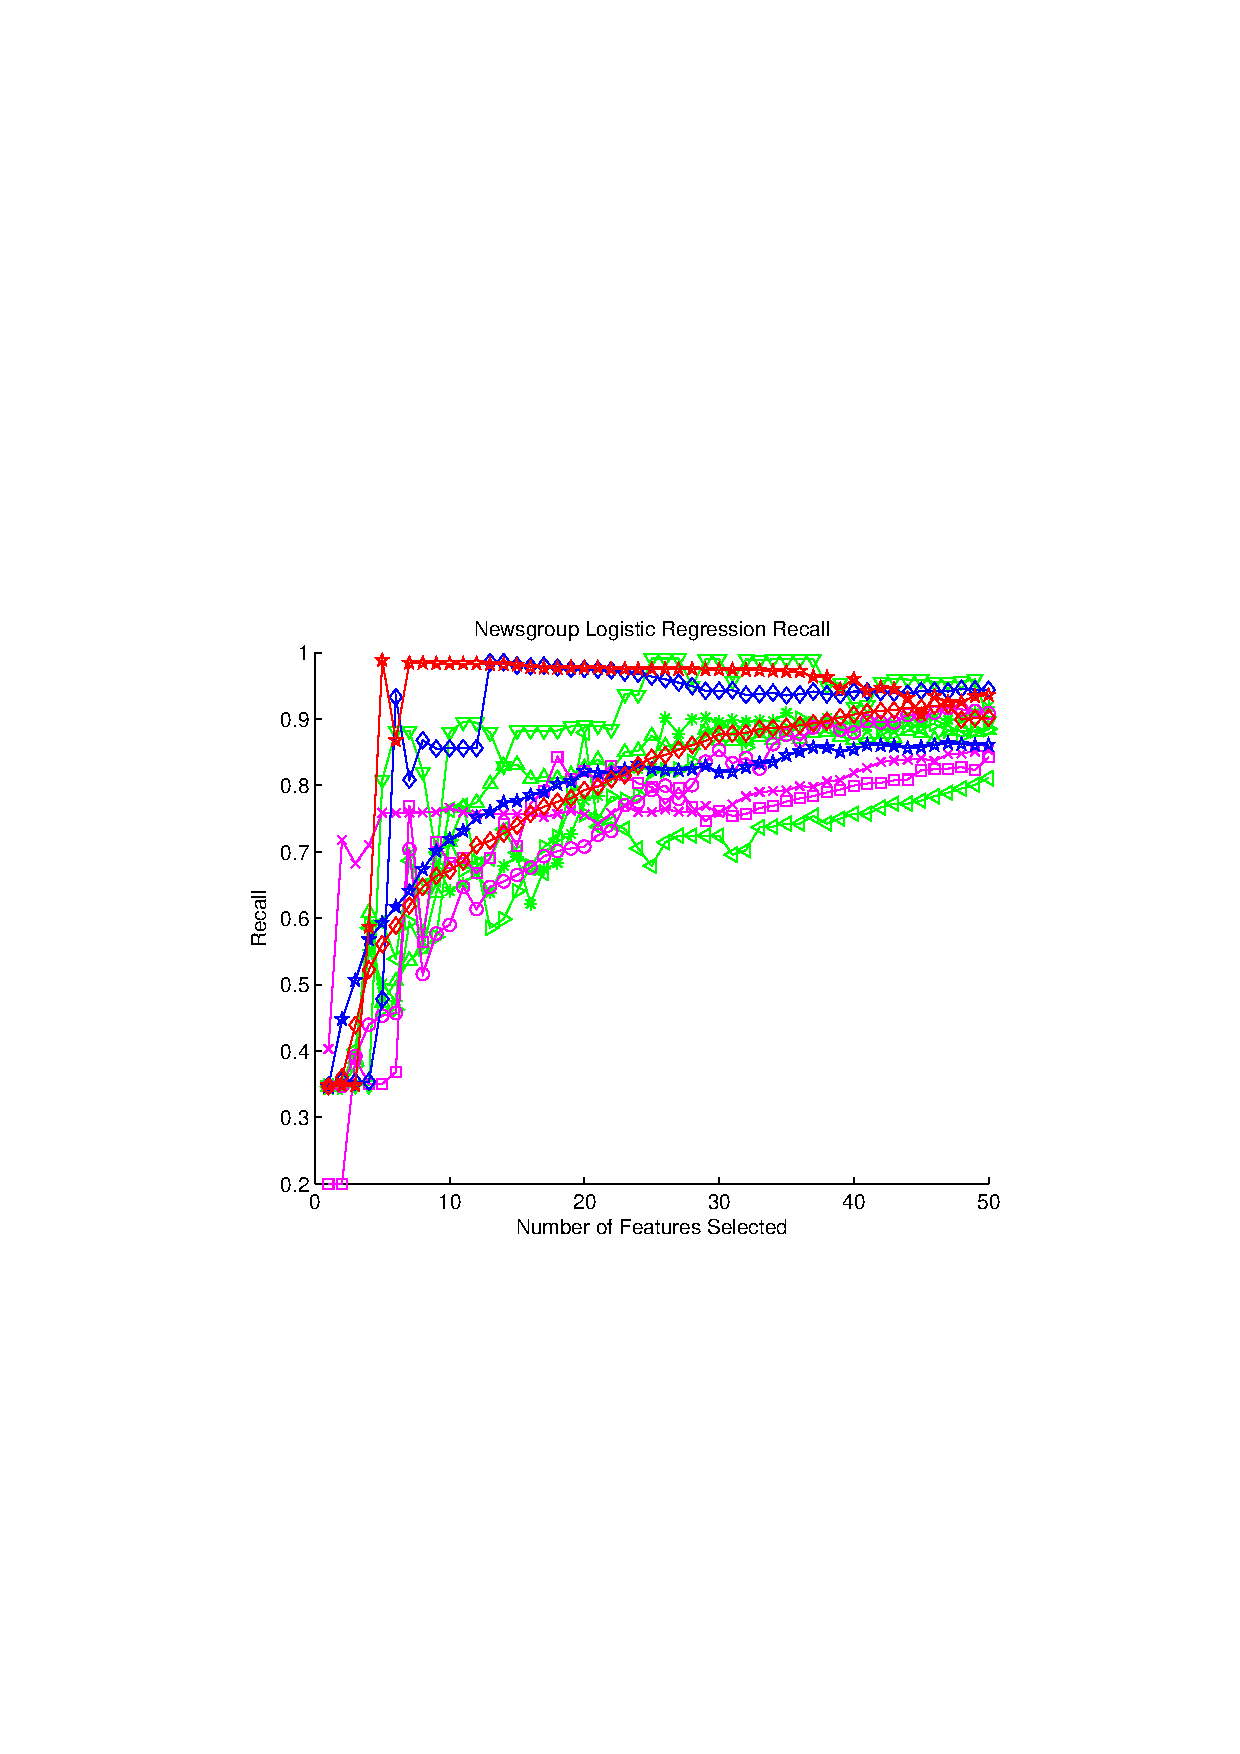
\includegraphics[width=0.375\textwidth]{./figures/linegraphs/NewsgroupLogisticRegressionRecall.pdf}
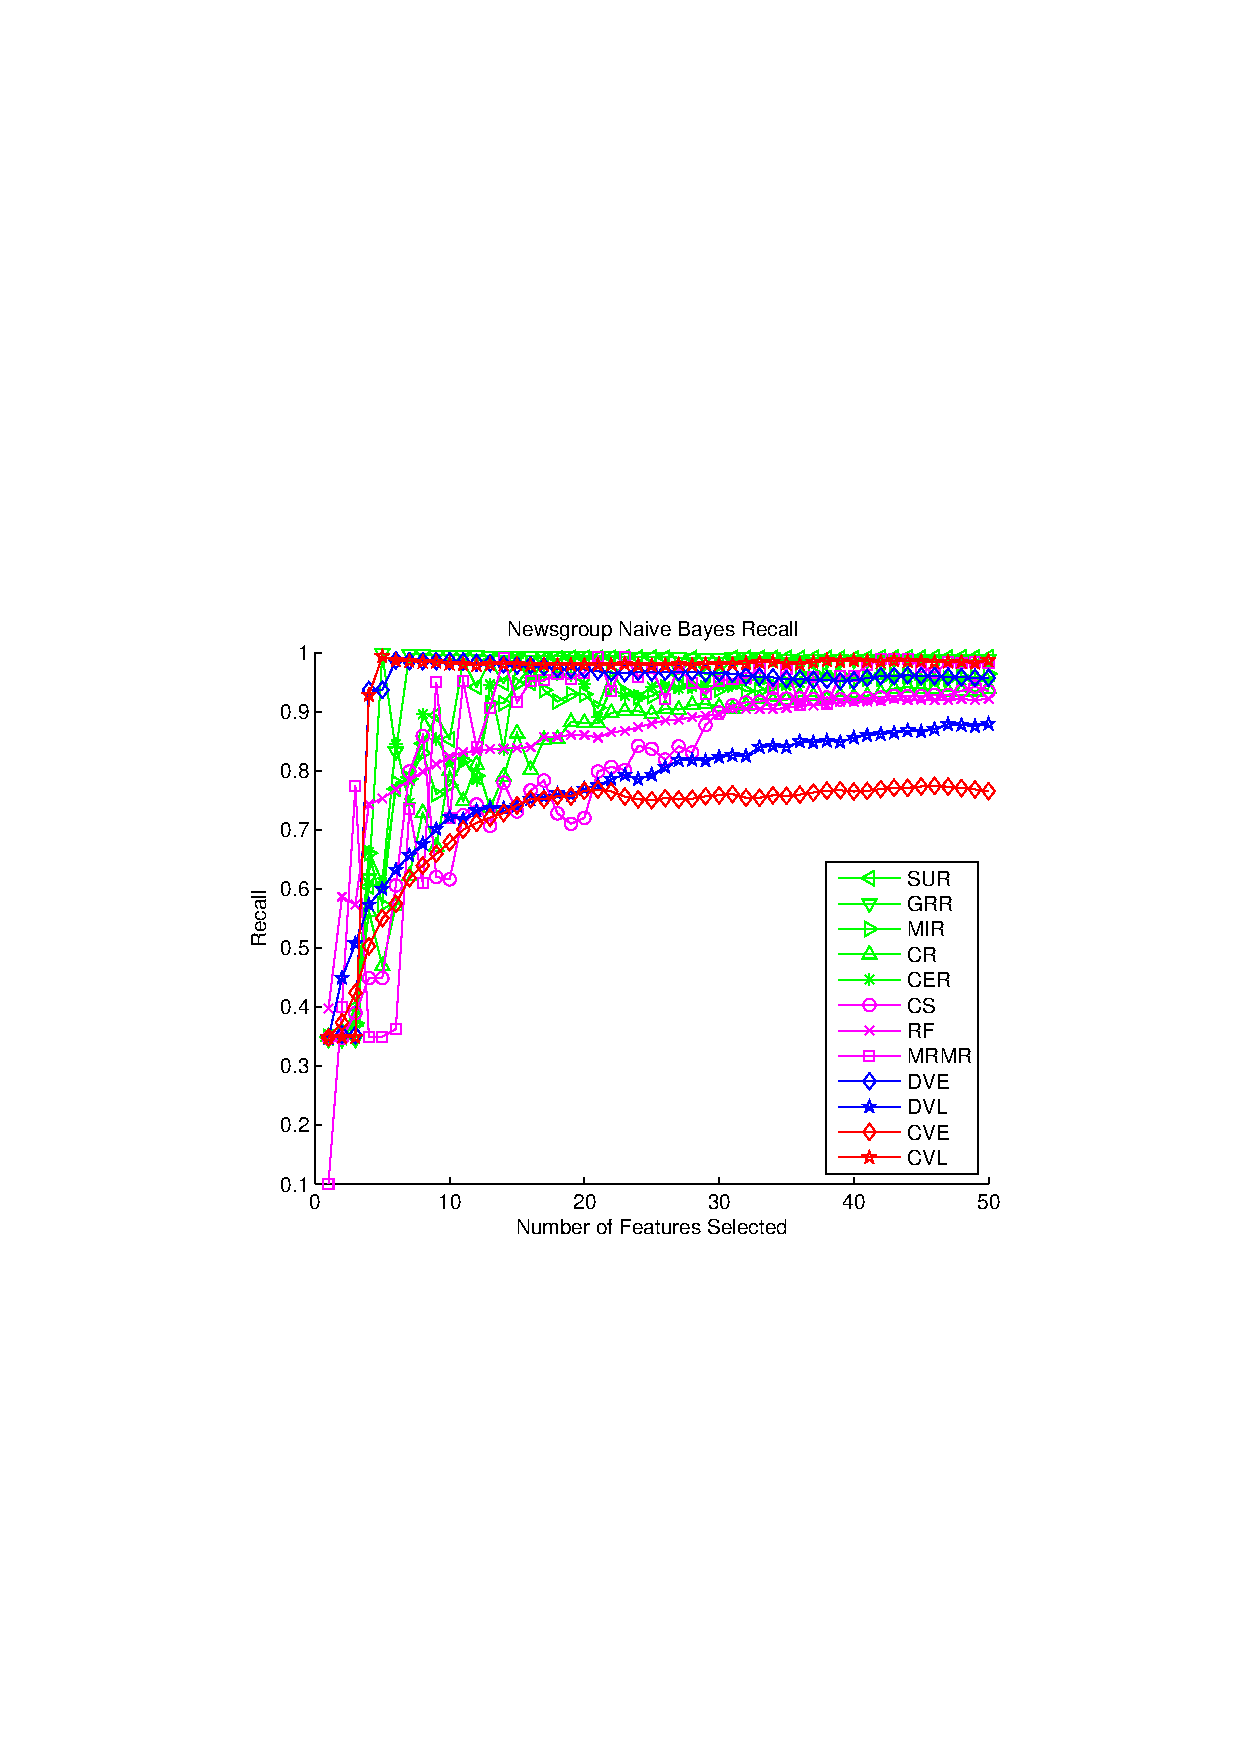
\includegraphics[width=0.375\textwidth]{./figures/linegraphs/NewsgroupNaiveBayesRecall.pdf}
%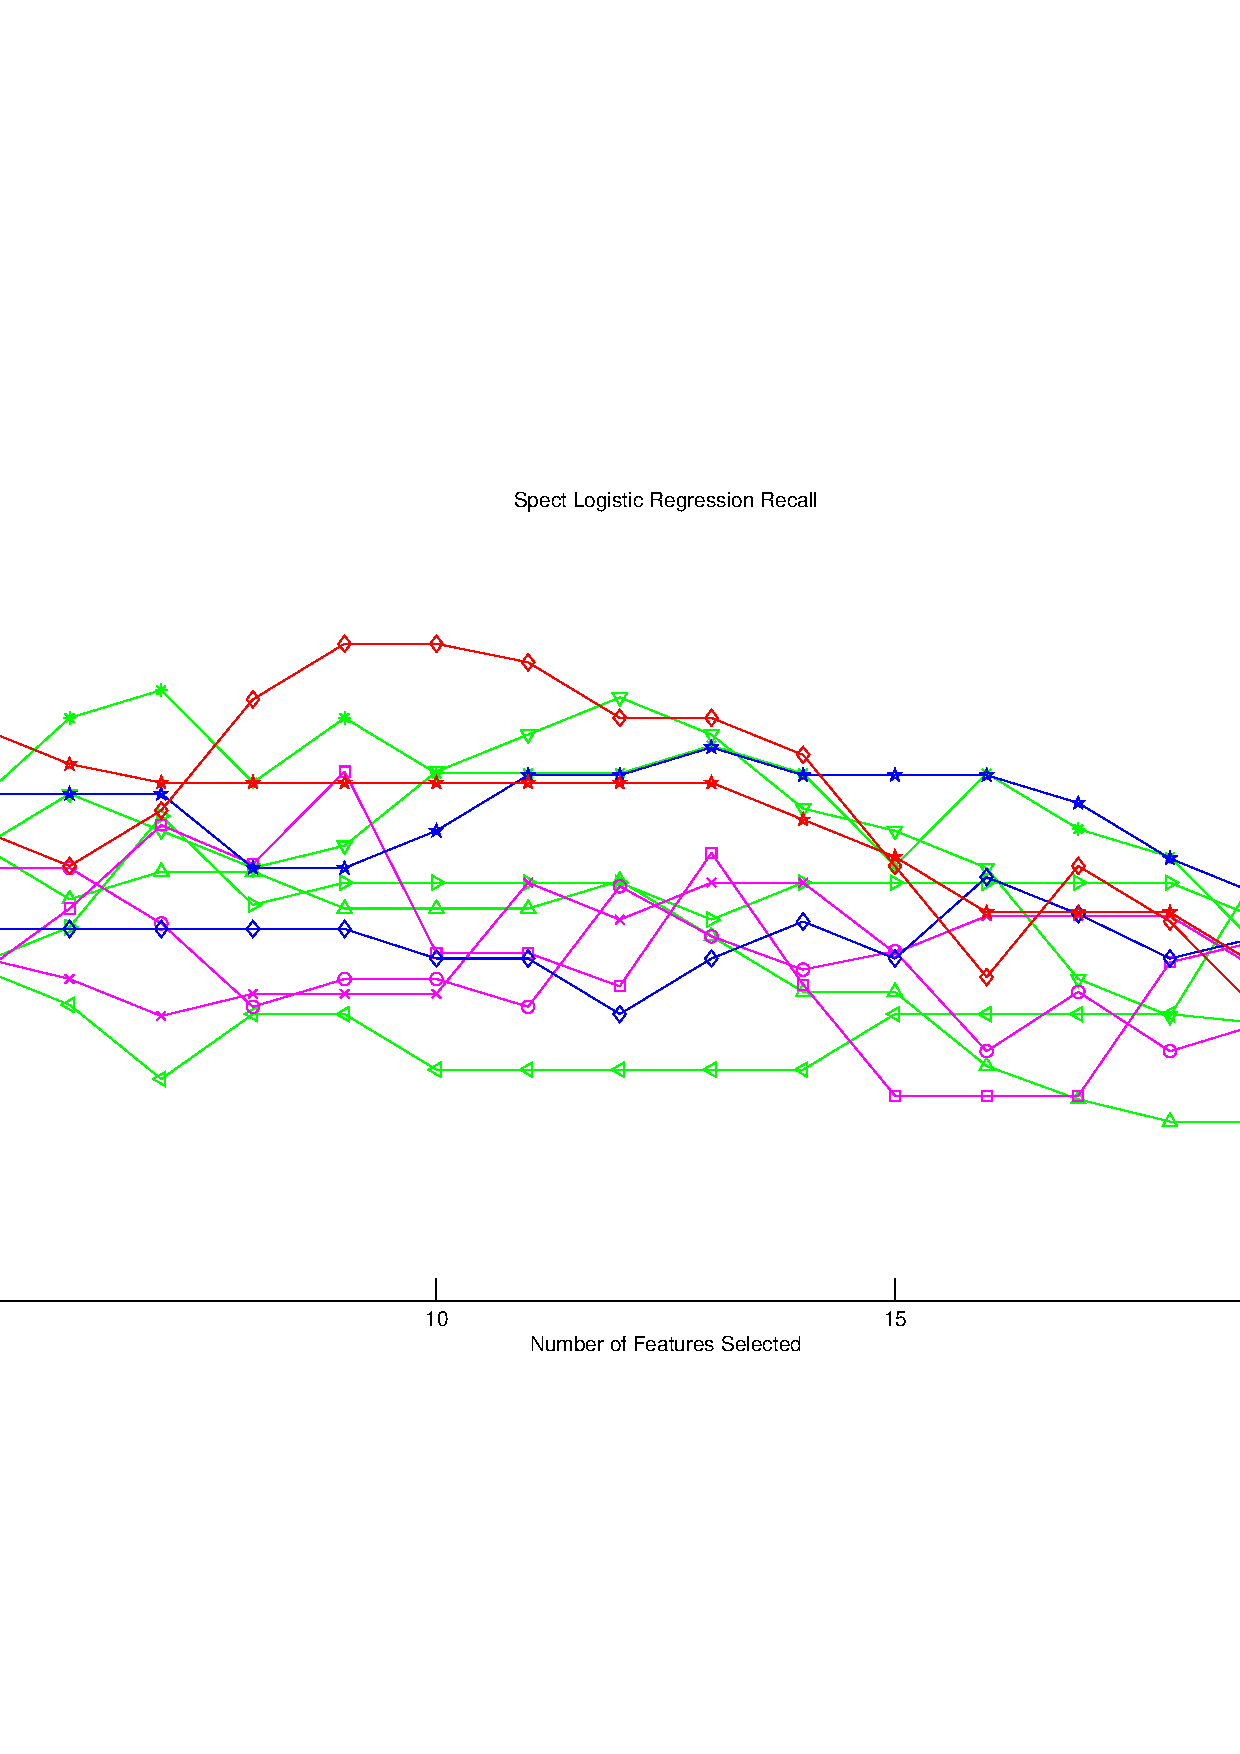
\includegraphics[width=0.375\textwidth]{./figures/linegraphs/SpectLogisticRegressionRecall2.pdf}
%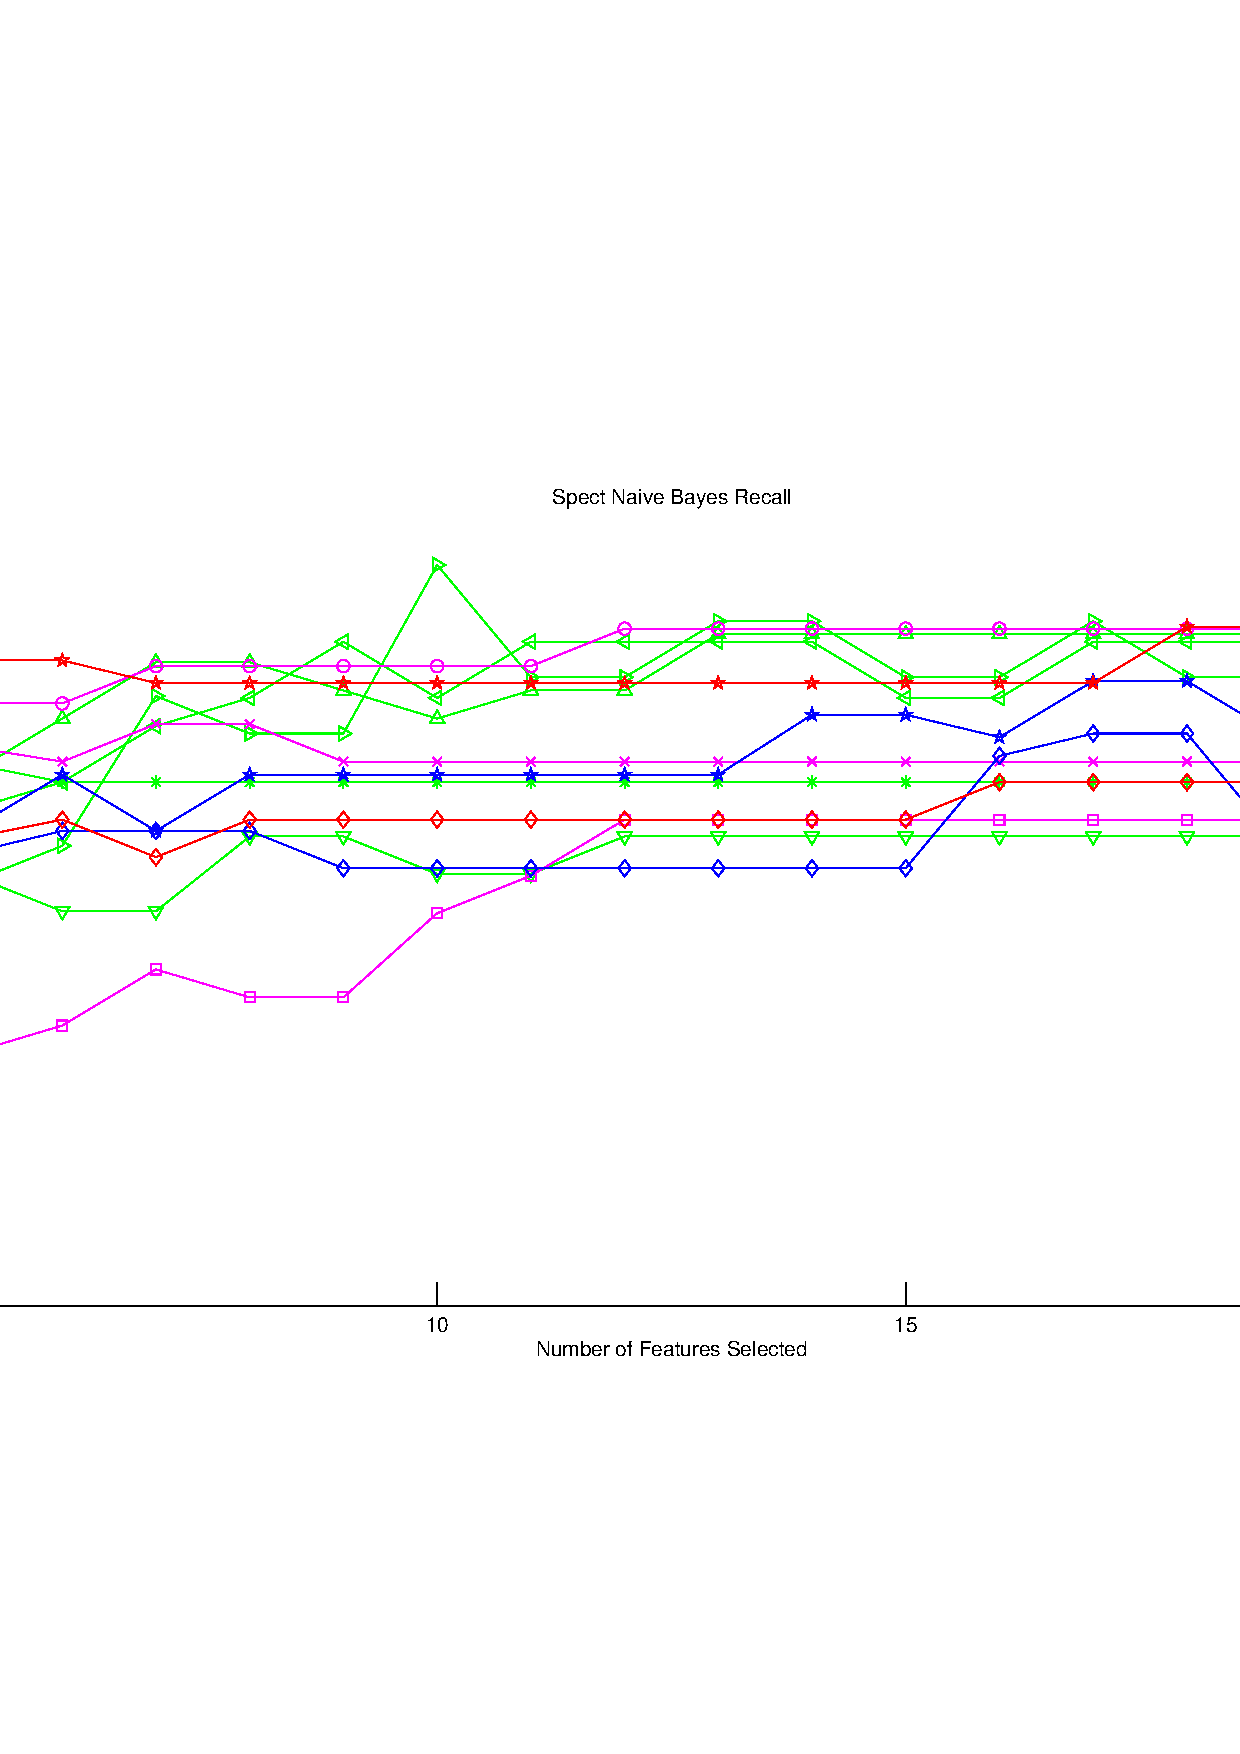
\includegraphics[width=0.375\textwidth]{./figures/linegraphs/SpectNaiveBayesRecall2.pdf}\\
%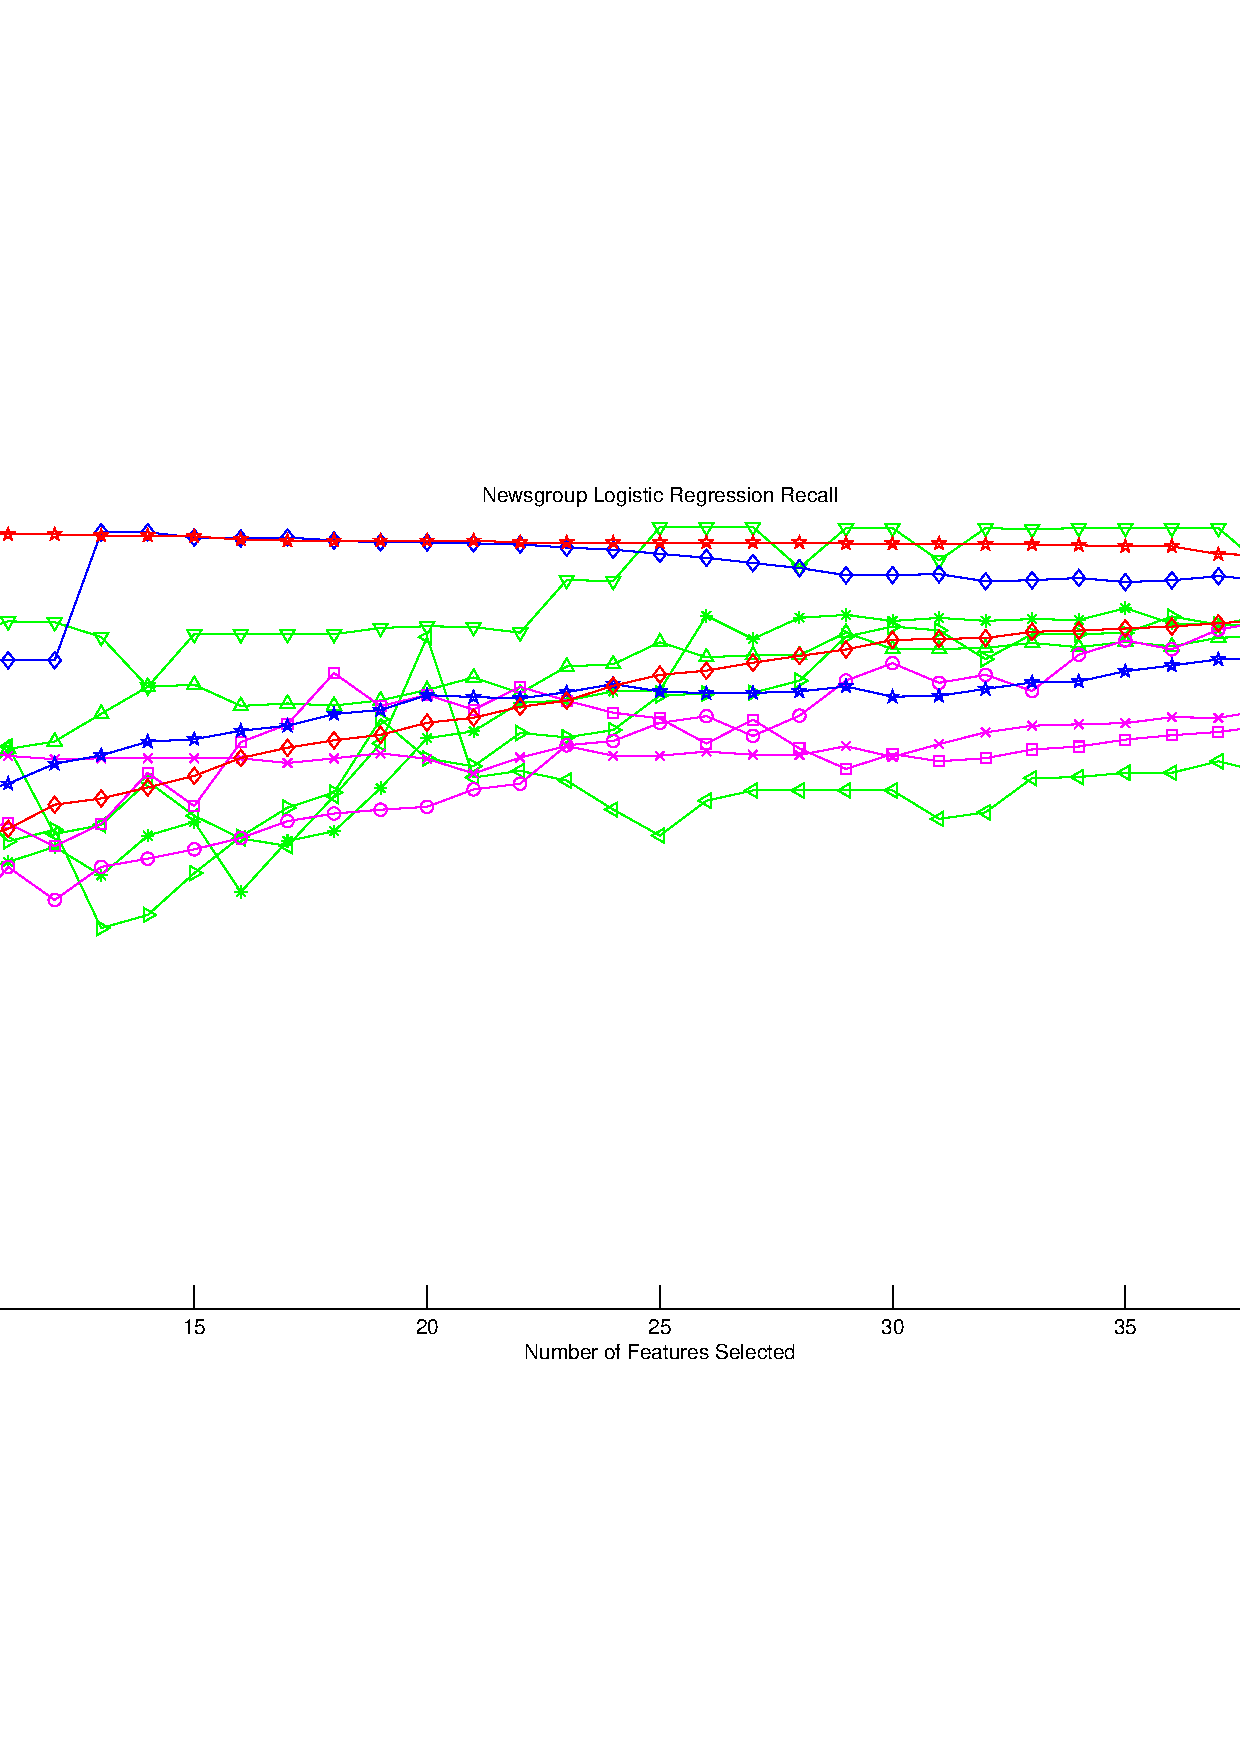
\includegraphics[width=0.375\textwidth]{./figures/linegraphs/NewsgroupLogisticRegressionRecall2.pdf}
%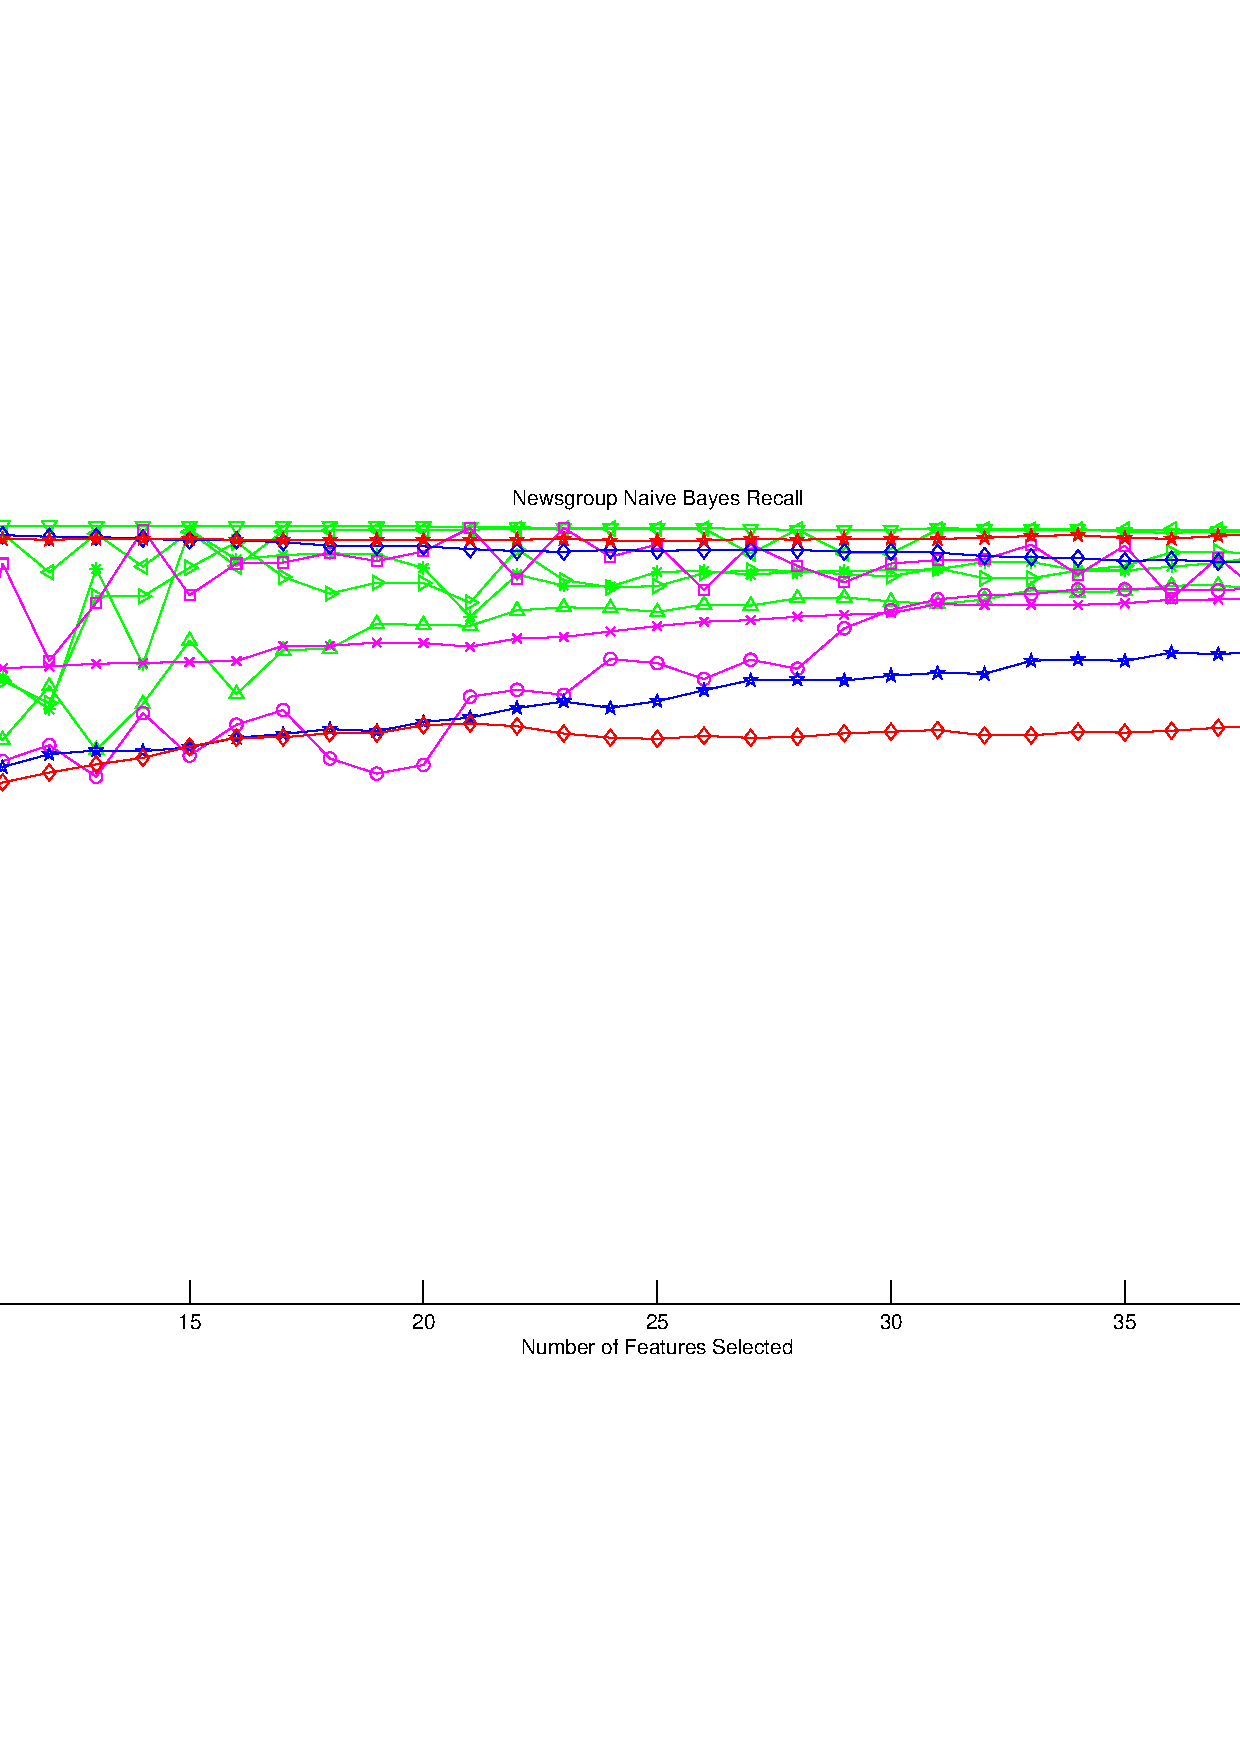
\includegraphics[width=0.375\textwidth]{./figures/linegraphs/NewsgroupNaiveBayesRecall2.pdf}
\caption{\footnotesize Performance distribution of various feature selection algorithms for two datasets and classifier types at each stage of feature selection.  The conjunctive voting methods do best overall in these datasets.}
\label{fig:perf_vs_fs_alg}
\end{figure*}
%%%%%%%%%%%%%%%%%%%%%%%%%%%%%%%%%%%%%%%%%%%%%%%%%%%%%%%%%%%%%%%%%%%%%%%%%%

\section{Empirical}

In this section, we conduct experiments to study the feature selection
performances of several well known methods such as Symmetrical
Uncertainty Rank (SUR), Gain Ratio Rank (GRR), Mutual Information Rank
(MIR), Correlation Based Rank (CR), Conditional Entropy Rank (CER)~\cite{guyon_jmlr03}, Correlation-based Feature Subset Selection (CS)~\cite{Hall1998}, Reliff (RF)~\cite{Robnik-Sikonja2003} , Minimum Redundancy Maximum Relevancem(MRMR)~\cite{peng2005} and our proposed methods:  Disjunction Voting Expectation(DVE) and  Disjunction Voting likelihood (DVL), Conjunction Voting Expectation (CVE), Conjunction Voting likelihood (CVL). The first five methods are variable rank methods and the last seven are subset rank methods. The first five methods are variable rank methods that select variables by ranking them with some metric and the last seven are subset rank methods that assess subsets of variables and consider previous selections to decide the next selection.

In this experimental study, we evaluated each feature selection
method on a variety of binary classification problems 
from the UCI machine learning repository \cite{Bache+Lichman:2013}.
These datasets along with their properties are outlined in 
Table~\ref{table:stats}.

In addition, we used three different classifiers to solve each of the
binary classifier problem. Logistic Regression, SVM Linear and Naive
Bayes were used in the experiments and the first two are implemented
in the LibLinear library~\cite{REF08a} and the last one is implemented in
the Weka software~\cite{weka}.
 
To evaluate feature selection algorithm performance, we perform 
10-fold nested cross-validation (nesting for tuning hyperparameters of each classification
algorithm) and evaluate accuracy, precision, and recall at each stage of
feature selection from the first selected feature through to the maximum
(either 50 or the number of features in the dataset, whichever is smaller).
%and F-Score for the true label class, that
%could be identified by the context of the problem and usually be the
%class with least samples in the data set.

In our evaluation, we wish to answer the following questions:
Do different feature selection methods perform better with
each classifier or on each dataset in comparison to others?
How reliably do the different feature selection methods perform overall
in terms of their performance distribution?
%\item Do any dataset features seem to correlate with algorithm performance?

To answer these questions, we first start with
Figure~\ref{fig:perf_vs_dataset}, where we evaluate the performance of
various feature selection algorithms per dataset, averaged across
classifier type and each stage of feature selection. We can observe that our approaches improve recall and accuracy in many of the binary classification problem.
% TODO Scott

In Figure~\ref{fig:perf_vs_classifier}, we examine how well our 
novel feature selection algorithms DVE, DVL, CVE, CVL 
perform vs. classifier, noting that overall performance is best
for Naive Bayes followed by Logistic Regression and noticeably worse for
the SVM Linear --- it seems simply that the probabilistic nature of our feature selection
dovetail best with classification methods that are themselves probabilistic,
and overall best with Naive Bayes which makes the same independence assumptions.

Next we examine Figure~\ref{fig:perf_vs_fs_alg}, where we evaluate the
performance distribution of various feature selection algorithms with
samples taken for each dataset, classifier type, and stage of feature
selection. This graph shows that our CVL high recall feature selection approach 
improves recall with the most improvement noticeable when there is a high
feature to data ratio such as in the Newsgroup (NG) and Spect (S) data
sets.  We conjecture the reason for this stems from the strong agreement of
features provided by the conjunctive voting scheme that helps reduce noise
in the feature selection process.

